\newcommand{\evolvemf}{\code{evolve\_mf}}



\section{Data}


We use a wide range of data to constrain the parameters of our models. In general, for both 47\,Tuc
and NGC\,3201 we use archival kinematic data from ground based spectroscopy, number density profiles from
\emph{Gaia} and stellar mass function data from HST photometry.

\subsection{Kinematics and density profiles}

\subsubsection{Proper motion dispersion profiles}

For 47 Tuc, we use two sets of {\it Hubble Space Telescope} (HST) proper motion data that are not
available for NGC\,3201. To probe the inner regions of the cluster we use the proper motion
dispersion profiles (both tangential and radial components) from \citet{Watkins2015} which are based
on a catalogue of proper motions of bright stars from \citet{Bellini2014}. These dispersion profiles
are built from stars brighter than the main sequence turn-off ($0.85 \ \mathrm{M}_\odot$ and $0.8 \
	\mathrm{M}_\odot$ for 47\,Tuc and NGC\,3201). To probe the kinematics in the outer regions of the
cluster, we also use the data from \citet{Heyl2017}, for which the mean mass of the measured stars
is $0.38 \ \mathrm{M}_{\odot}$. The outer proper motion data also allows us to constrain the amount
of radial anisotropy present in the cluster, which can mimic the effect of central dark mass in
isotropic models by raising the central velocity dispersion \citep{Zocchi2017}.


\subsubsection{Line-of-sight velocity dispersion profiles}

For both 47\,Tuc and NGC\,3201 we use the line-of-sight velocity dispersion profiles from
\citet{Baumgardt2018} to further constrain the kinematics of the clusters. These dispersion profiles
are based on archival ESO/VLT and Keck spectra along with previously published radial velocity data
from the literature. As these radial velocity samples are dominated by bright stars, we assume that
the velocity dispersion profile traces the kinematics of upper main-sequence and evolved stars in
our models.

\subsubsection{Number density profiles}
We use the number density profiles from \citet{DeBoer2019} to constrain the size and structural
parameters of the clusters. These profiles are made up of a combination of cluster members based on
Gaia DR2 data in the outer regions and data from various literature sources in the central regions.
The Gaia data used only includes bright stars ($m > 0.6 \ \mathrm{M}_\odot$, for both clusters) and
the literature data is dominated by bright stars, therefore in our models we assume the profiles
probe the distribution of upper main sequence and evolved stars.

\subsection{Stellar mass functions}

As a constraint on the global present-day stellar mass function of the clusters, we use a
compilation of HST based stellar mass function data from
Baumgardt\footnote{\url{https://people.smp.uq.edu.au/HolgerBaumgardt/globular/}} (2021, priv.
comm.), which represent an updated and augmented version of the stellar mass functions found in
\citet{Sollima2017}. This compilation is made up of several HST fields at varying distances from the
cluster centre. These fields extend out to $14 '$ and $8.33 '$ from the cluster centres for 47\,Tuc
and NGC\,3201 respectively and cover a mass range of $0.16 - 0.8 \ \mathrm{M}_\odot$. The large
radial and mass ranges allow us to constrain the degree mass segregation in the clusters.

\subsection{Pulsar Data}

For 47\,Tuc, we make use of its large population of millisecond pulsars (MSPs) to place further
constraints on its mass distribution. We use both the spin and orbital period timing solutions from
\citet{Freire2017}, \citet{Ridolfi2016} and \citet{Freire2018}. We also consider the dispersion
measures of the pulsars which, when combined with internal gas models from \citet{Abbate2018}, allow
us to constrain the line-of-sight position of the pulsars within the cluster. The work surrounding
the use of pulsar data to constrain the models was performed as part of an earlier project and so
will not be discussed in too much detail in this project.



\subsection{Binary Data}

In order to create realistic binary populations we use the data from \citet{Milone2012} to inform
our choices of binary fraction and mass ratio distribution. For 47\,Tuc this means a flat mass
ration distribution and a binary fraction of roughly $2\%$ \ps{This is so small, do we want to use
	something larger for testing the effects?}.  For NGC\,3201 \citet{Milone2012} find a binary fraction
of around $10\%$ with a flat mass ratio distribution while \citet{Giesers2019} find a value closer
to $f_b = 0.0675$ without constraining the mass ratio distribution.





\section{Generating mass functions}

The bulk of project deals with generating mass functions to use as inputs to the \code{LIMEPY}
models, we do this in two main steps, we first generate a present-day mass function comprised of
only single stars, and we then modify it to include binary stars.

\subsection{Single Star Mass Functions}

\ps{More details here?}

To generate the mass functions comprised of single stars we use the \evolvemf{} algorithm from
\code{SSPTools}\footnote{\url{www.github.com/pjs902/ssptools}}, a publicly available package for
working with simple stellar populations.

The \evolvemf{} algorithm combines precomputed grids of stellar evolution models and isochrones to
accurately model the evolution of a given initial mass function, fully including the effects of
stellar evolution, mass loss due to escaping stars and dynamical ejections. The algorithm returns a
sampled mass function for a requested time, ideal for use in the \code{LIMEPY} models.

We parameterize the mass function as a broken power-law with breakpoints at $0.5 \mathrm{M}_\odot$
and $1.0 \mathrm{M}_\odot$. We provide to \evolvemf{} the initial mass function slopes and
breakpoints, the cluster age, metallicity and escape velocity, as well as parameters which control
the mass loss due to escaping stars the specific binning to be used when the present day mass
function is sampled. Figure \ref{fig:2/evolve_mf} shows the evolution of a mass function over a
span of $10 \ \mathrm{Gyr}$.

\begin{figure}
	\centering
	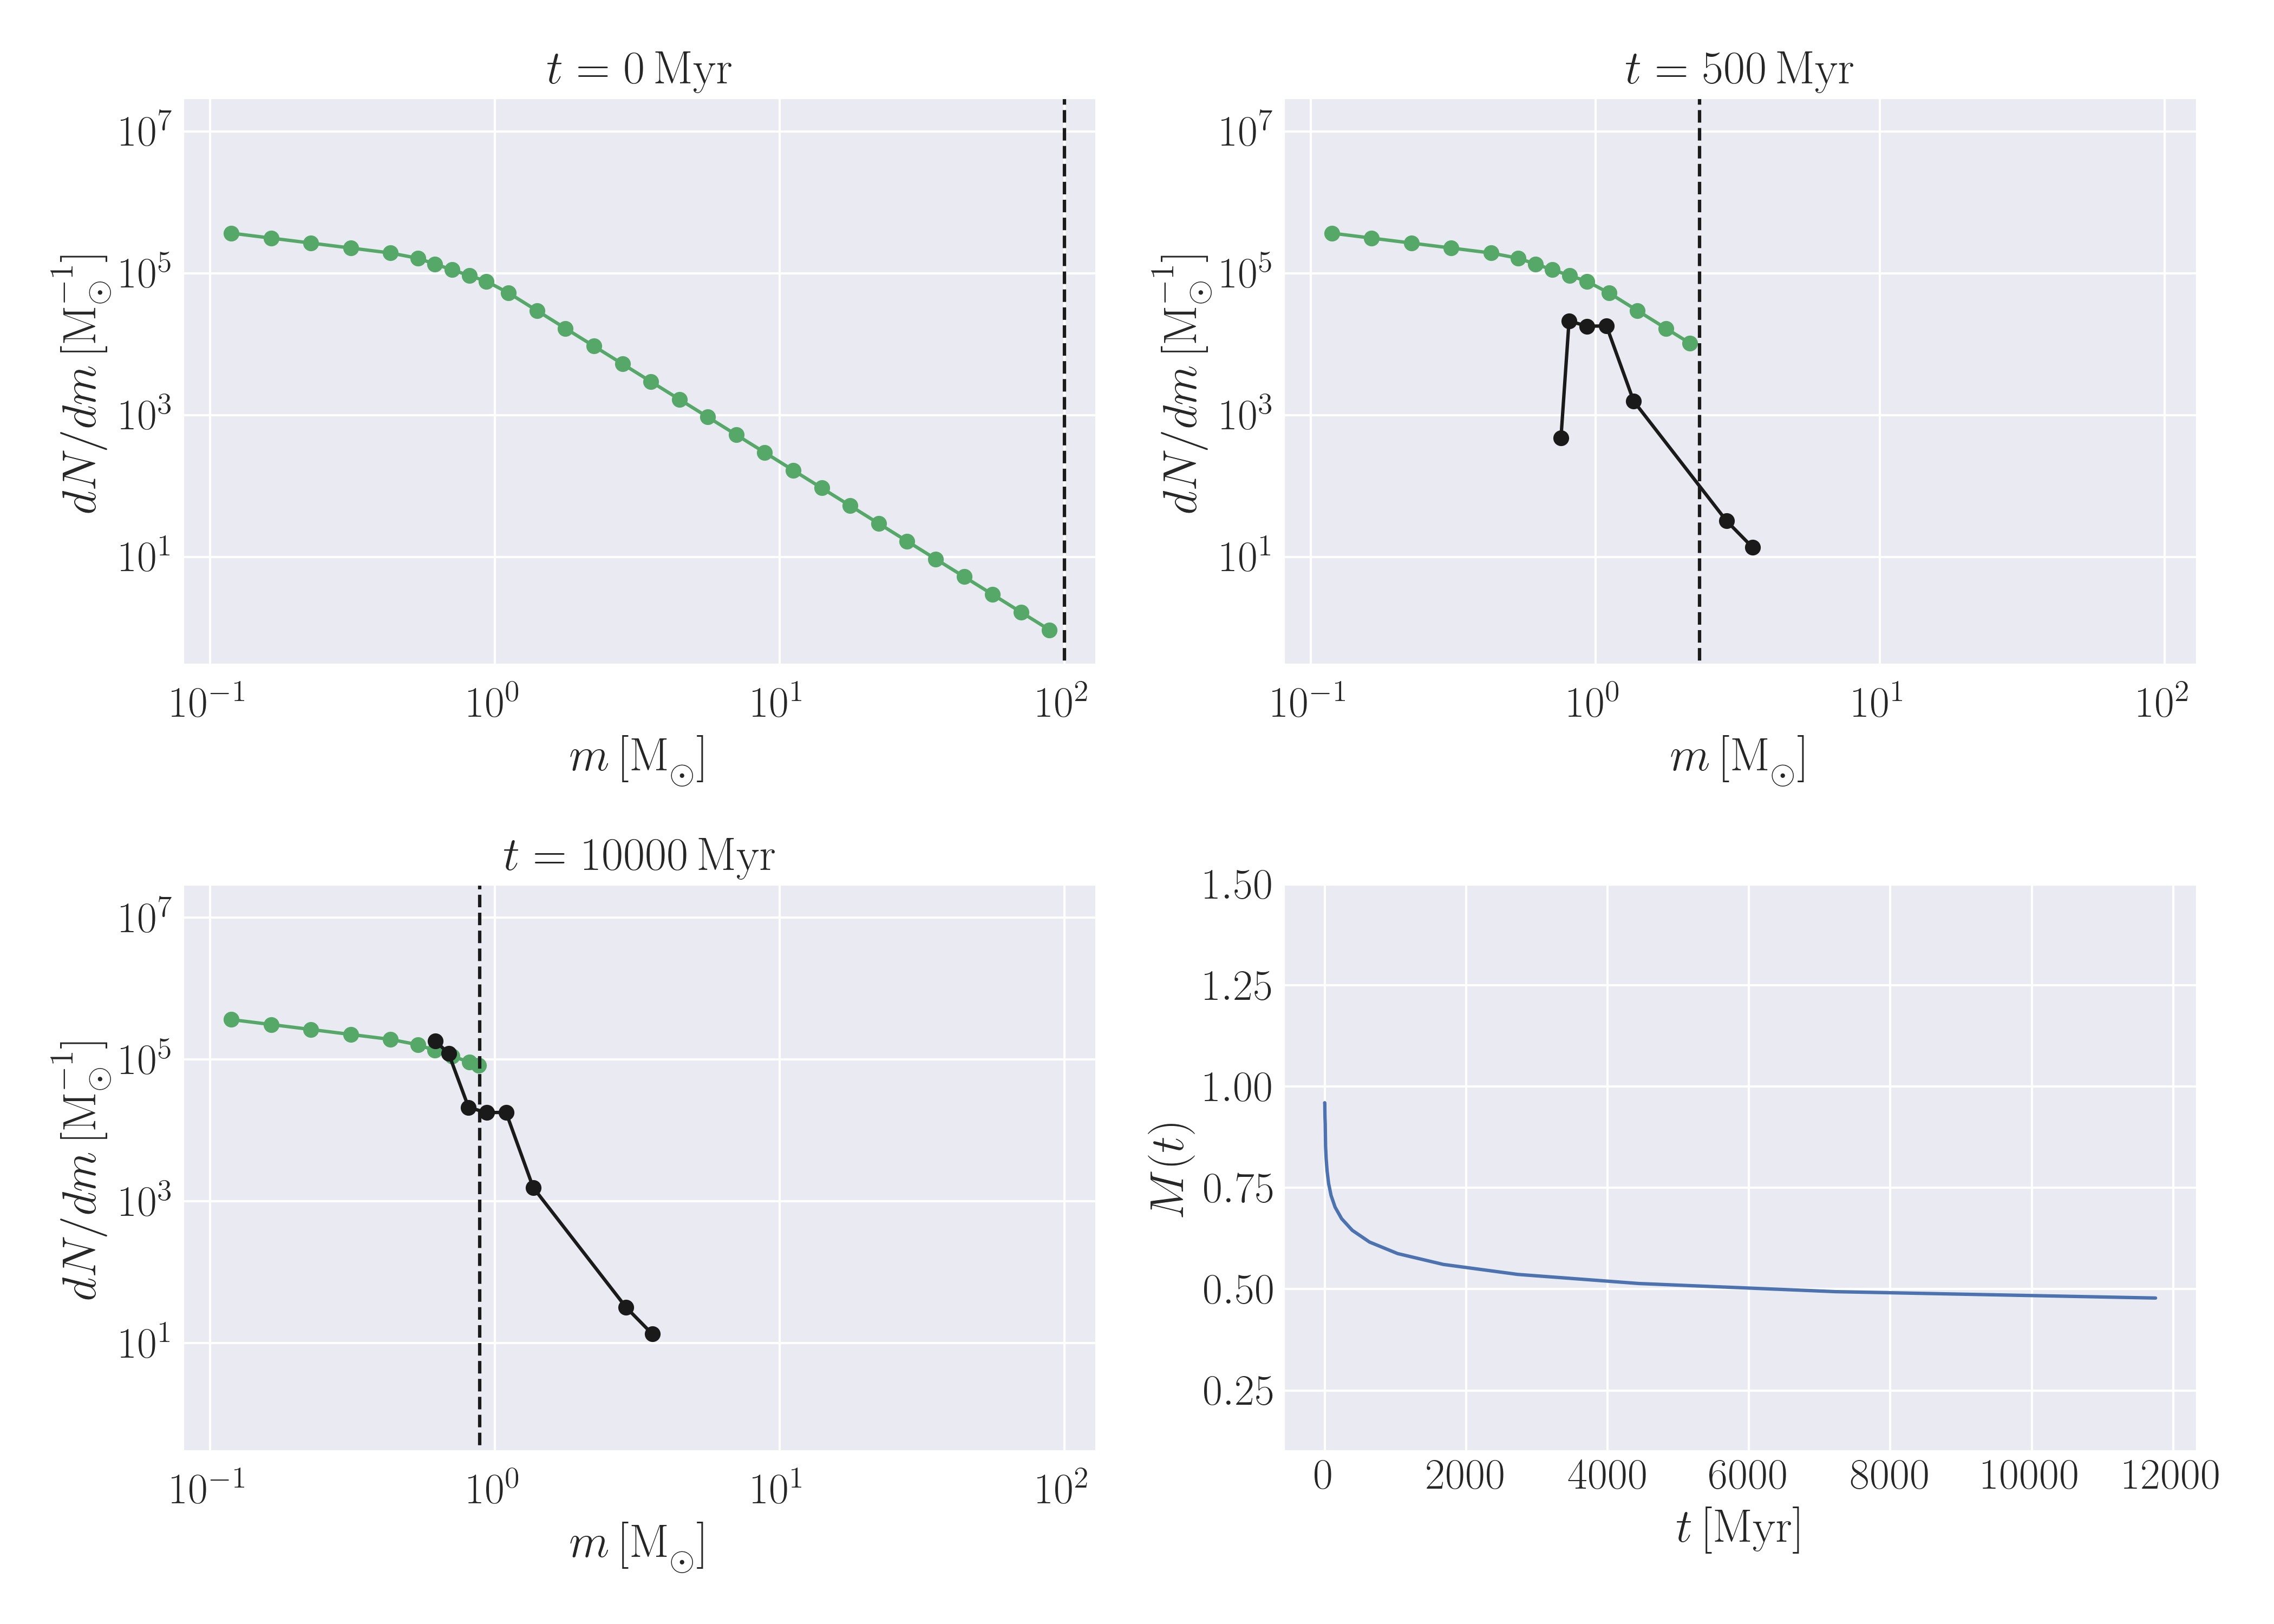
\includegraphics[width=\textwidth]{figures/evolve_mf.png}
	\caption{The evolution of a typical mass function from $t=0$ to $t=10000 \ \mathrm{Myr}$.
		The stellar bins are plotted in green while the remnant bins are plotted in black,
		the current main-sequence turn-off is plotted a dashed black line. As the mass
		function ages, more and more main sequence stars evolve into remnants. Lower right:
		The evolution of the total mass of the mass function is plotted as a fraction of the
		initial mass. Mass loss is dominated by the effects of stellar evolution but also
		has contribution from dynamical ejected and escaping stars.}
	\label{fig:2/evolve_mf}
\end{figure}


\subsection{Binary Mass Functions}

In order to include binary stars in our mass functions we make use of the assumption that for the
vast majority of their interactions with other objects, binary systems behave essentially as point
masses given the fact that they are tightly bound. This means that in order to replicate the effects
of a binary population in our mass function, we simply need to shift some of the mass in single
stars into heavier bins which act as the "binary bins".


We split this process up into several steps. First we divide the total binary fraction among the
values if $q$ in the requested mass ration distribution. We weight the $f_b$ values assigned to the
individual values of $q$ by the chosen mass ration distribution, so a flat mass ratio distribution
would have the total binary fraction divided evenly among the values while a "solar distribution"
(see \citealt{Fisher2005}) would have a significantly higher portion of the total $f_b$ assigned to
equal mass binaries. Figure \ref{fig:2/q-dists} shows the resulting mass ratio distributions using
this method.

\begin{figure}
	\centering
	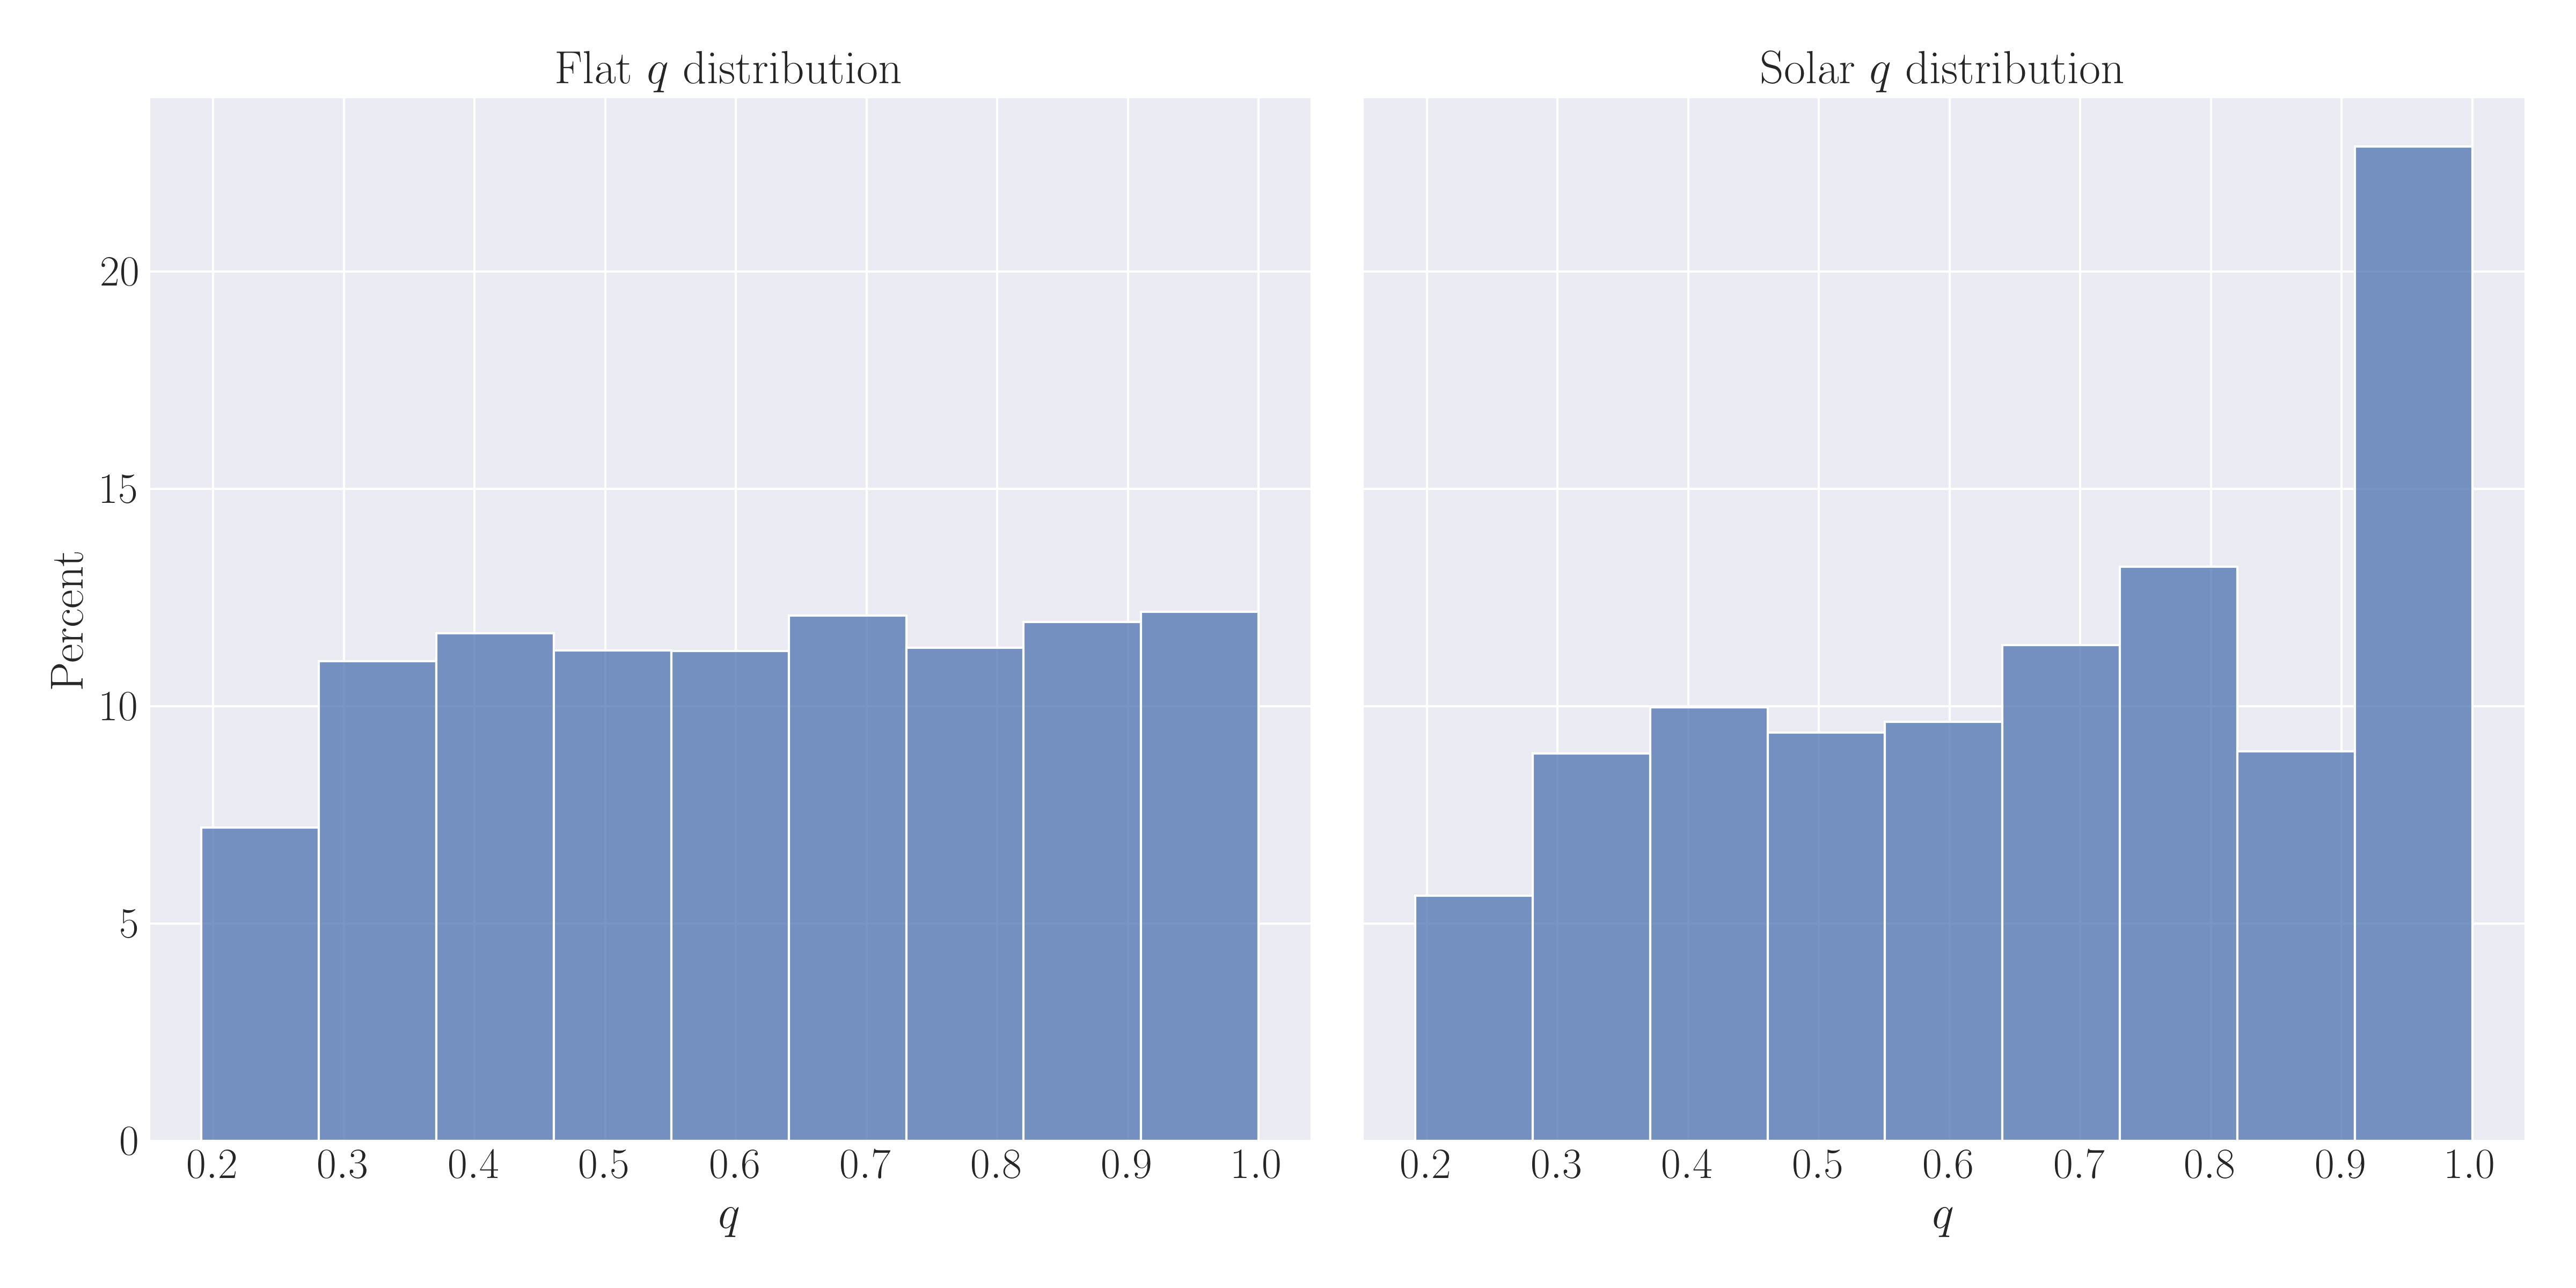
\includegraphics[width=\textwidth]{figures/q-dists.png}
	\caption{The resulting mass ratio distributions for the "flat" and "solar" mass ratio
		prescriptions. Both distributions are truncated and lowered at $q=0.2$ due to the
		relative lack low very low mass stars within the mass functions, making the creation
		of very low $q$ binaries impossible.}
	\label{fig:2/q-dists}
\end{figure}


After we have calculated the individual binary fractions for each value of $q$, we then go through
each bin of main sequence stars and attempt to make binaries. The companion mass for a given bin is
calculated using the current value of $q$ and the number of binaries to make is calculated using the
binary fraction for the current value of $q$. After the companion mass and number of binaries are
set, we then find the closest bin to the companion mass and subtract from the primary and companion
bins the mass corresponding to the calculated number of binaries, adding the subtracted mass to a
new bin with a mean mass equal to the sum of each binary component.


We repeat this process for each bin of main sequence stars until all bins have a binary fraction
equal to that of the current value of $q$. We do this process for each value of $q$ in the mass
ratio distribution, resulting in each main sequence bin having a binary fraction equal to the
requested total binary fraction and a mass ratio distribution identical to the requested
distribution.


This process tends to create on the order of 150 new bins in our mass function which dramatically
increases the runtime of the \code{LIMEPY} models. In order to prevent this we group together binary
bins of similar masses, forming on the order of 15 binary bins containing binary systems of similar
total mass but differing mass ratios. Figure \ref{fig:2/shifted-mf} shows the original main sequence
bins, plotted with the modified main sequence bins, binary bins and rebinned binary bins.


\begin{figure}
	\centering
	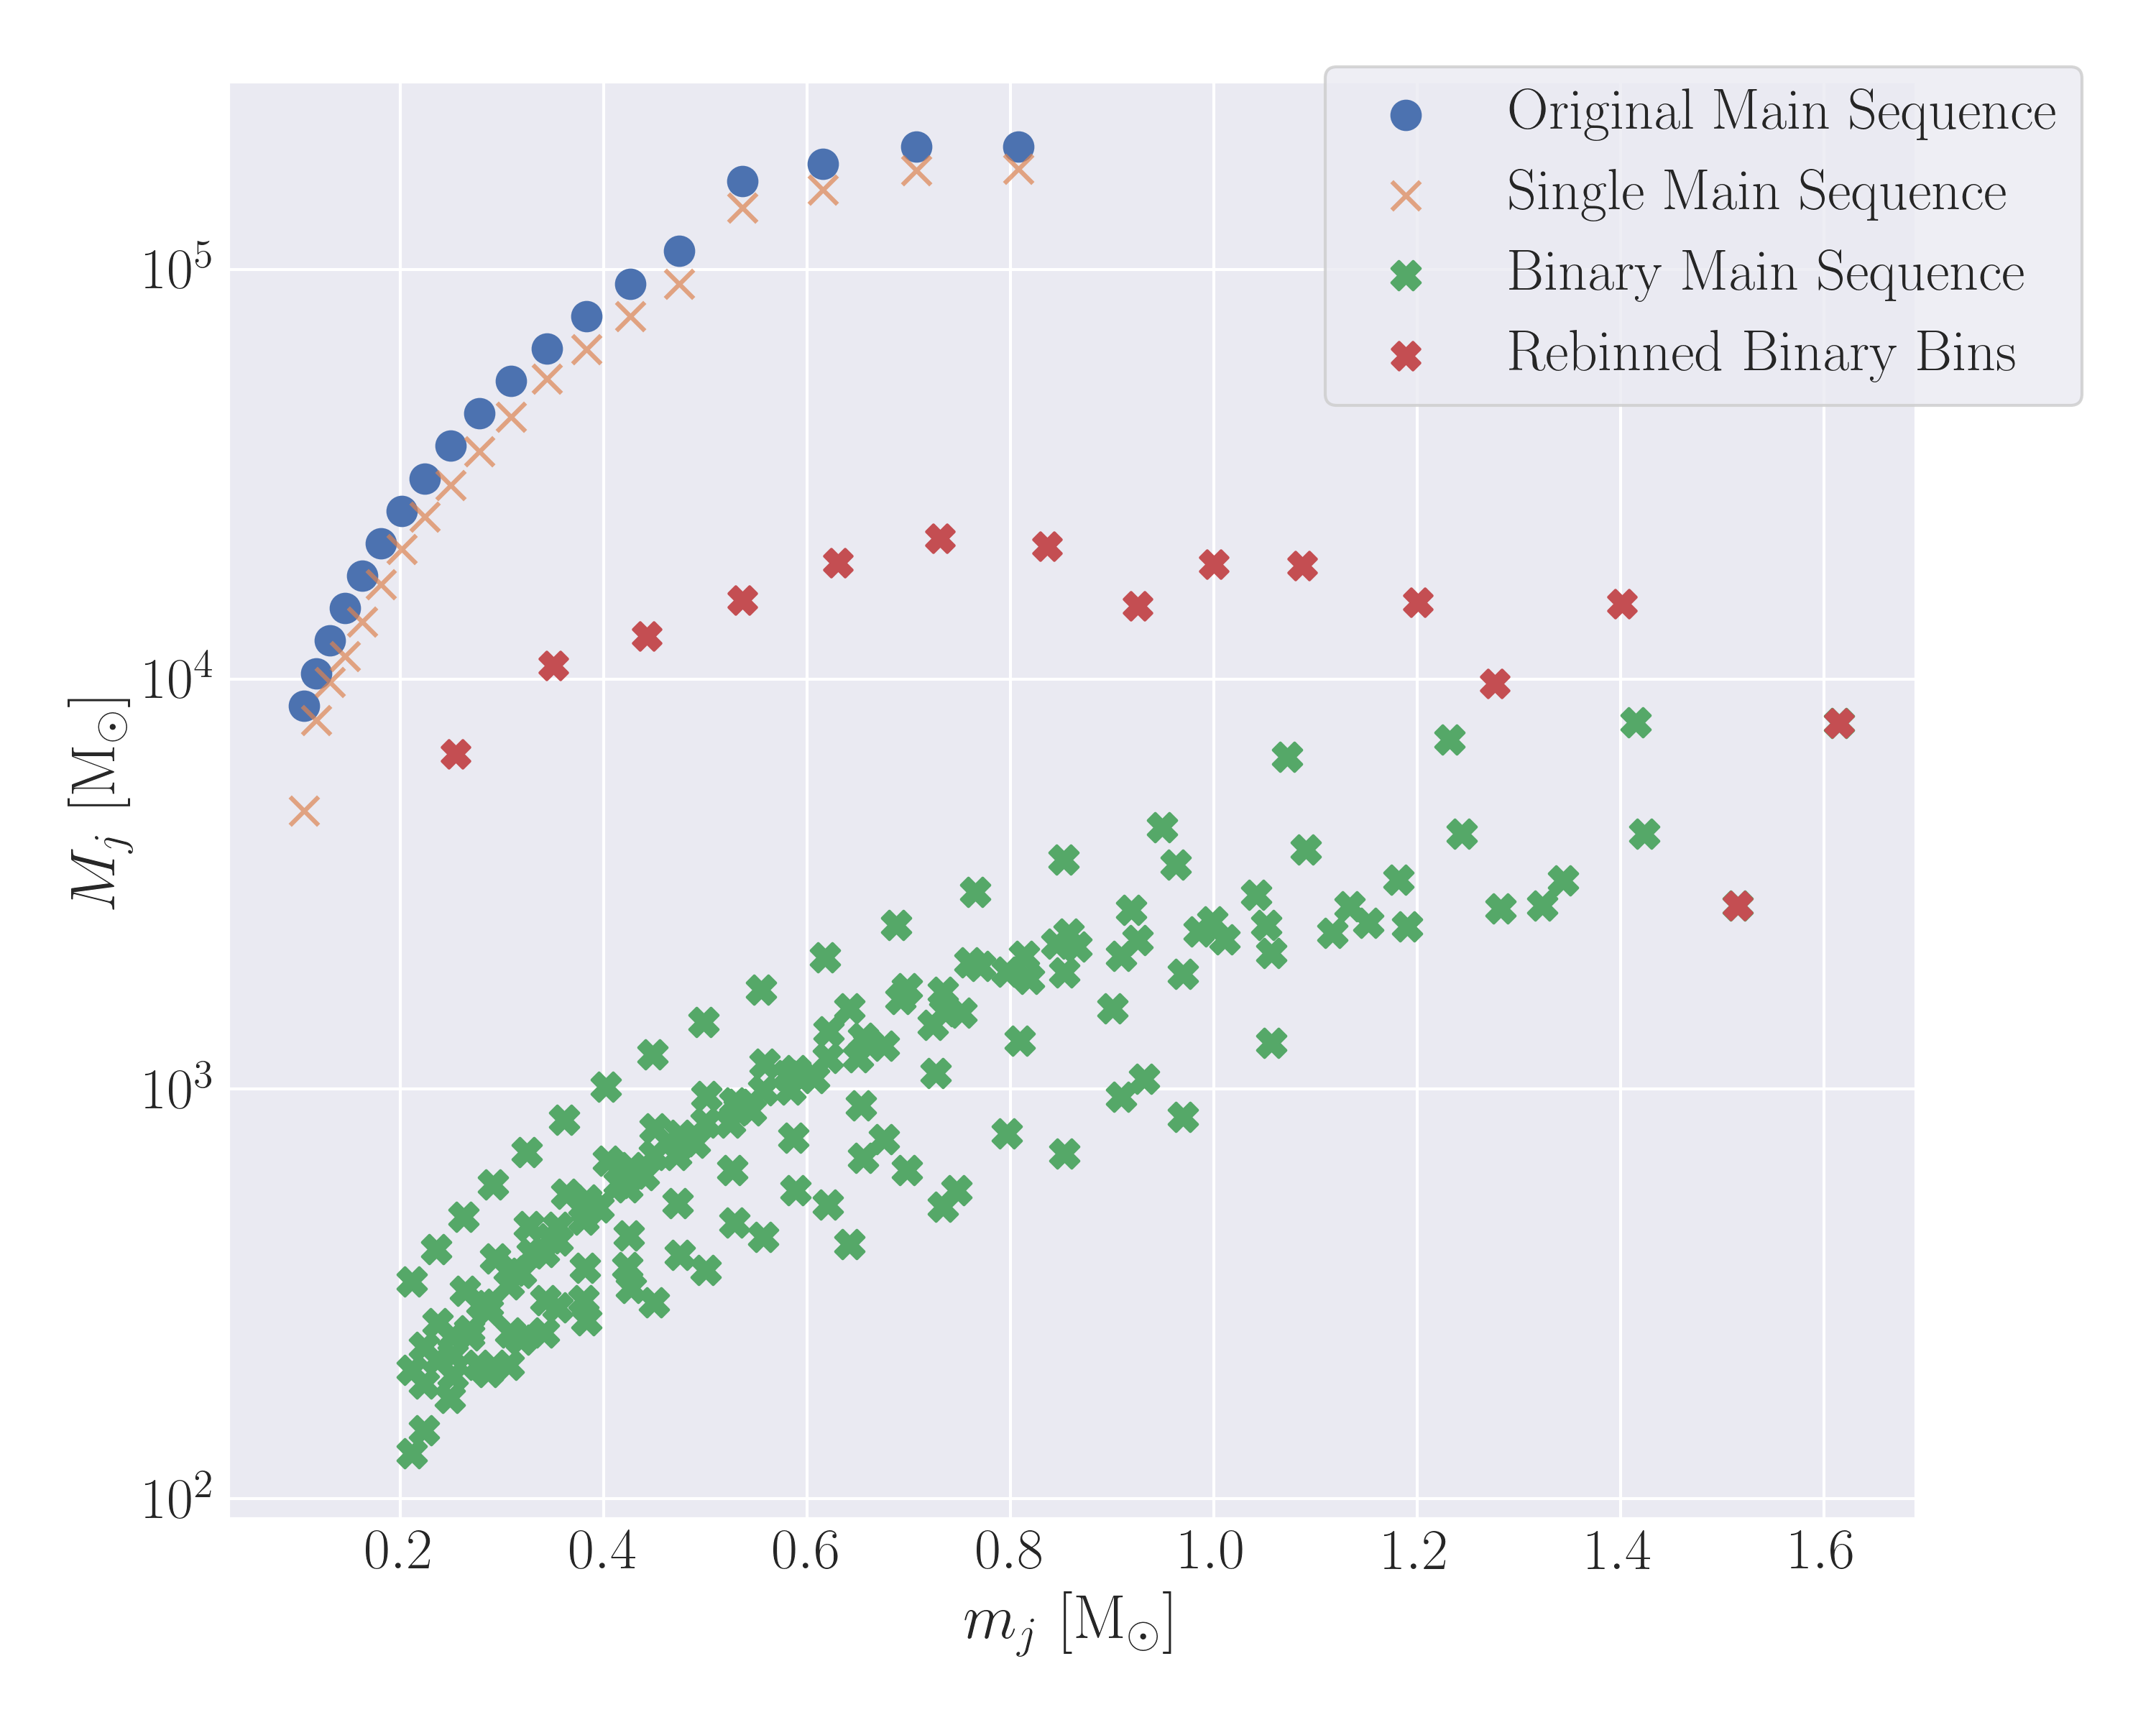
\includegraphics[width=0.8\textwidth]{figures/shifted-mf.png}
	\caption{The main-sequence portion of a mass function before and after binaries are added.
		The blue circles are the original main sequence and the crosses are the modified main
		sequence. The orange crosses show the single stars after mass has been removed to create
		binaries and the many green crosses are the binary bins that are initially created. The red
		crosses are the rebinned binary bins which are actually used in the computation of the
		\code{LIMEPY} models.}
	\label{fig:2/shifted-mf}
\end{figure}



\section{Fitting Models to Data}


To fit our models to the data we use the \code{GCfit}
package\footnote{\url{www.github.com/nmdickson/gcfit}}. \code{GCfit} provides a uniform interface
for fitting \evolvemf{} and \code{LIMEPY} models to observations of clusters using either MCMC or
Nested Sampling.

\ps{Here we should say if we use Nested Sampling or MCMC and why  and what the setup is like.}

\subsection{Likelihoods}

The majority of the likelihood functions we use are simple Gaussian likelihoods of the following form:

\begin{equation}
	\ln \left(\mathcal{L}\right)=\frac{1}{2}
	\sum_{r}\left(\frac{\left(\sigma_{\mathrm{obs}}(r)
		-\sigma_{\mathrm{model}}(r)\right)^{2}}{\delta \sigma_{\mathrm{obs}}^{2}(r)}
	-\ln \left(\delta \sigma_{\mathrm{obs}}^{2}(r)\right)\right)
\end{equation}

Where $\mathcal{L}$ is the likelihood, $\sigma$ is the line-of-sight velocity dispersion, $r$ is the
projected distance from the cluster centre, and $\delta \sigma$ is the uncertainty in the velocity
dispersion. The likelihoods for other observables are formulated in the same way, and the specifics
are discussed in \code{GCfit}'s documentation\footnote{\url{gcfit.readthedocs.io}}. The total
likelihood is therefore the sum of all the log-likelihoods for each set of observations.

For the mass function and number density likelihoods we include additional nuisance and scaling
terms to account for extra sources of error in the mass function data and the effects of potential
escapers at the cluster boundary.




\subsection{Fitting Mass Functions to Observations}

When the mass function data was originally collected, the mass was recorded based on the position of
the star on an isochrone fit to the cluster. This means that any binary stars in the sample are
recorded as single stars a mass corresponding to a star with the average colour of the two binary
components and a luminosity corresponding to the sum of the two components.

Additionally, when we move mass around to create binary bins we remove mass from the surface density
profiles which would be compared to the mass function data. In order to compensate for these
effects, we rescale the surface density profiles to include the stars which are in binary bins,
according to how they would have been observed using the observational method described above.

In order to determine the observed mass we use a grid of MIST isochrones computed at a range of
metallicities, at the age of the cluster. We use the isochrone to determine the luminosity of the
binary components and then use the isochrone to determine the observed mass of the combined
luminosities. We then scale the surface density profile of the main sequence bin which most closely
matches the observed mass of the binary system by the total mass of the binary system which allows
us to correct for both effects.